
\section{Additional Results} \label{AppendixA}

\subsection{Logistic regression for assistance applications}

Below we report logistic regression results for the applicant status, that is whether a county applied for federal disaster assistance based on the Public Assistance Applicants Program Deliveries data. This is regressed on a few variables, including the share of democratic votes in the 2016 election. The other independent variables are also from 2016.

Similarly, the declaration status, that is whether a county had any natural disasters declared during the 2009 to 2018 period. This is regressed on the share of democratic votes in the 2008 election and the set of same control variables.


\begin{table}[htbp]
   \centering
   \caption{\label{ResultsLogit} Determinants of Assistance Application}
   \begin{tabular}{lc}
      \tabularnewline\midrule\midrule
      Dependent Variable:        & Applicant\\
      Model:                     & (1)\\
      \midrule \emph{Variables} &  \\
      (Intercept)                & -3.622\\
                                 & (3.723)\\
      Share of democratic voters & -0.8362$^{**}$\\
                                 & (0.3469)\\
      Median Income (logs)       & 0.2939\\
                                 & (0.3331)\\
      Poverty Rate               & 4.033$^{**}$\\
                                 & (1.575)\\
      Share of single mothers    & 4.068$^{***}$\\
                                 & (1.144)\\
      \midrule \emph{Fit statistics} &  \\
      Observations               & 2,882\\
      Squared Correlation        & 0.02306\\
      Pseudo R$^2$               & 0.01966\\
      BIC                        & 3,724.7\\
      \midrule\midrule\multicolumn{2}{l}{\emph{IID standard-errors in parentheses}}\\
      \multicolumn{2}{l}{\emph{Signif. Codes: ***: 0.01, **: 0.05, *: 0.1}}\\
   \end{tabular}
\end{table}





\section{Pre-Treatment Trends} \label{PreTrends}

Here we show plots of aggregated pre-treatment trends to justify the parallel trends assumption. Mean test scores are aggregated by cohort (year of first treatment) and relative time to treatment, and never treated units act as the control group. We only display these plots for overall test scores for both datasets, but not for subgroups. However, the plots for the subgroups look very similar.

\begin{figure}[!h]
	\centering
	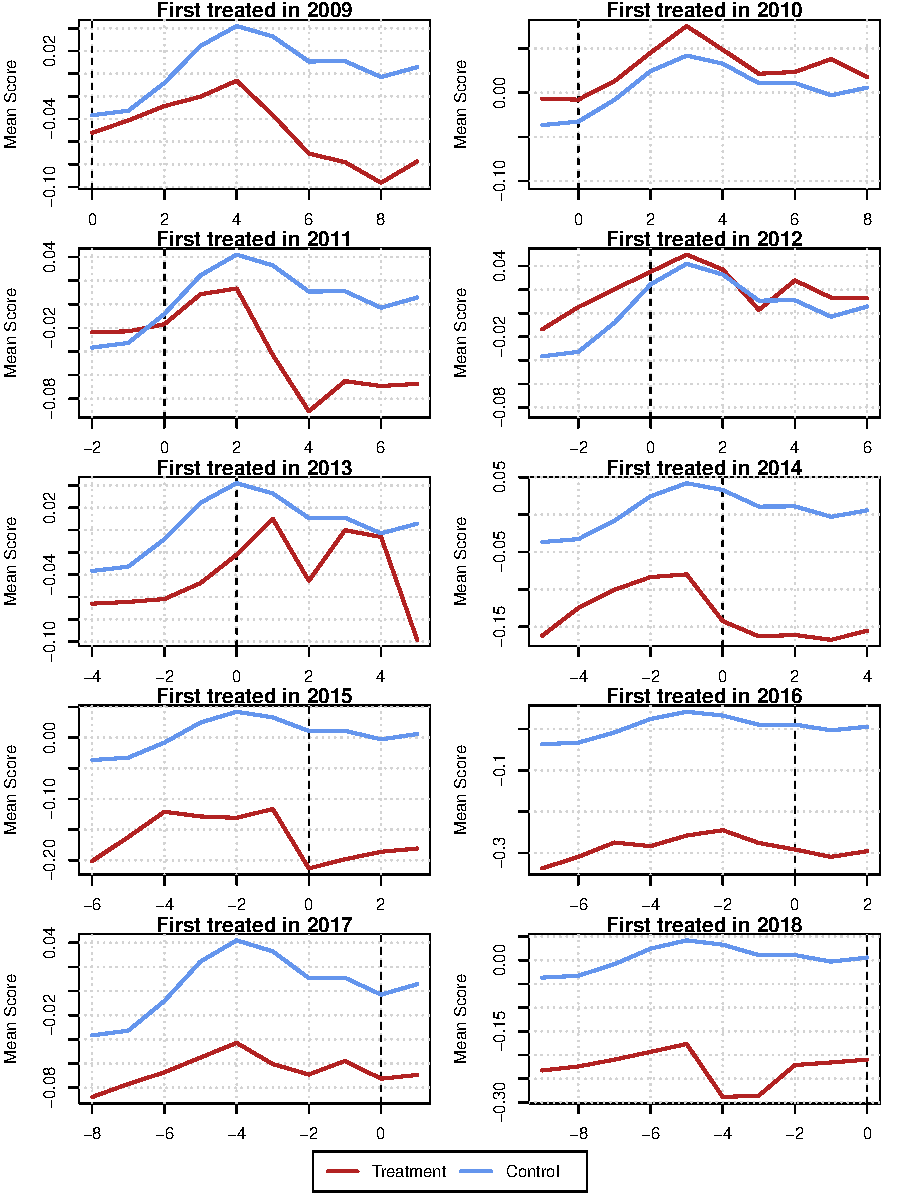
\includegraphics[scale=1]{"../Code & Data/ParTrendsPlotMathematicsFEMA.png"}
	\caption{Pre trends for aggregated mean scores in mathematics based on FEMA data}
	\label{PreTrendsMath}
\end{figure}

\begin{figure}[!h]
	\centering
	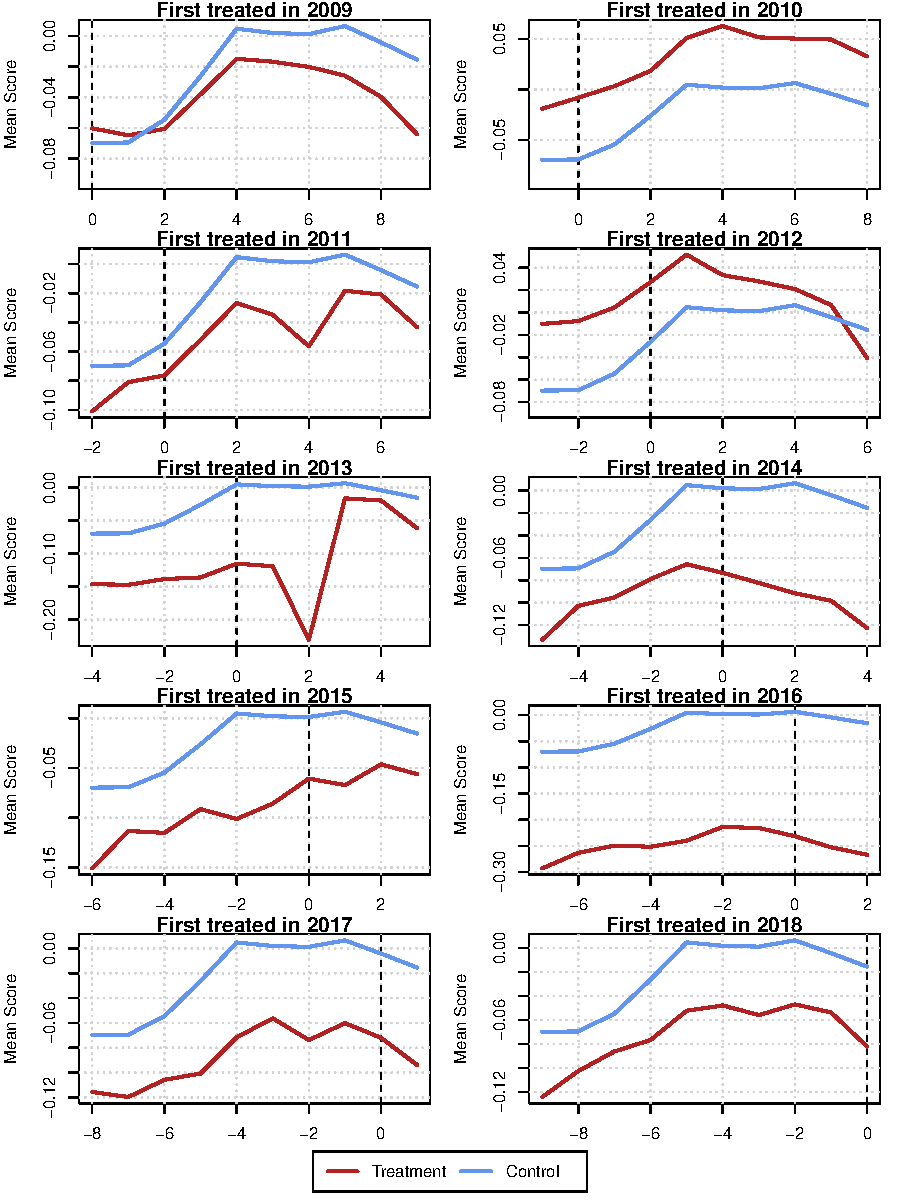
\includegraphics[scale=1]{"../Code & Data/ParTrendsPlotRLAFEMA.png"}
	\caption{Pre trends for aggregated mean scores in RLA based on FEMA data}
	\label{PreTrendsRLA}
\end{figure}

\begin{figure}[!h]
	\centering
	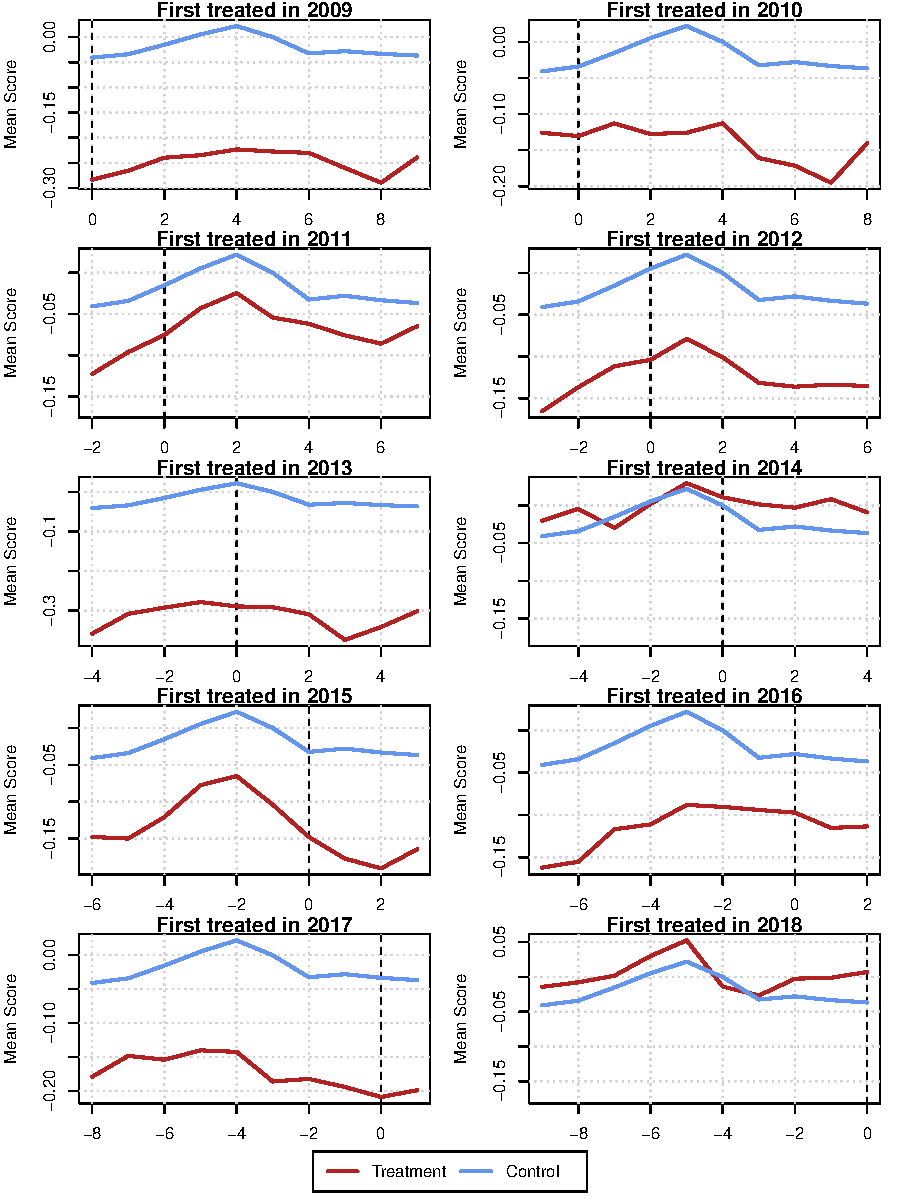
\includegraphics[scale=1]{"../Code & Data/ParTrendsPlotMathematicsStorm.png"}
	\caption{Pre trends for aggregated mean scores in mathematics based on NWS storm data}
	\label{PreTrendsMath}
\end{figure}

\begin{figure}[!h]
	\centering
	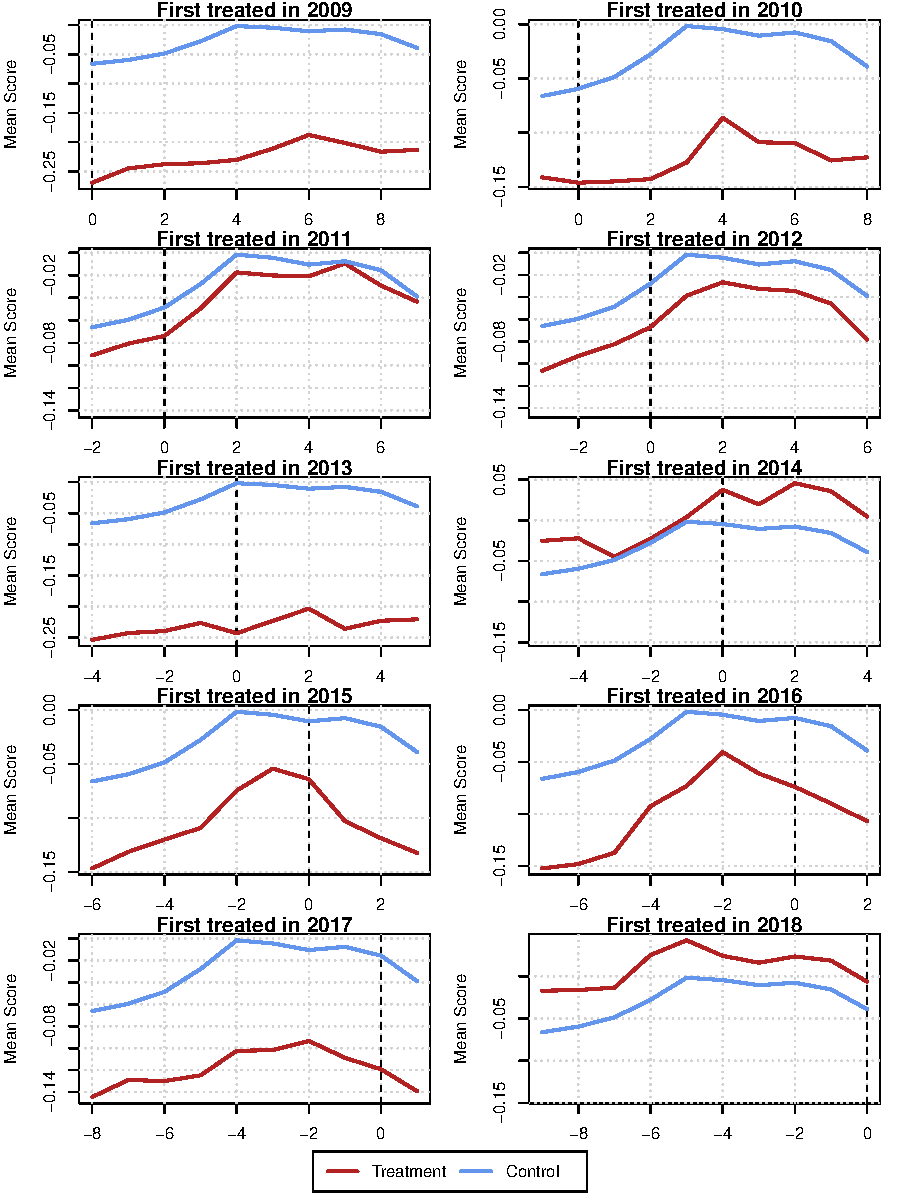
\includegraphics[scale=1]{"../Code & Data/ParTrendsPlotRLAStorm.png"}
	\caption{Pre trends for aggregated mean scores in RLA based on NWS storm data}
	\label{PreTrendsRLA}
\end{figure}



